% Generated by tools/rbq_fig_*.py from committed records. Do not edit by
% hand: regenerate instead, so the figure and its manifest entry stay in
% step. Records read are listed in
% experiments/mmsys2027_rbq_retarget_20260914/paper_figures_20260915/FIGURES_R1.json.
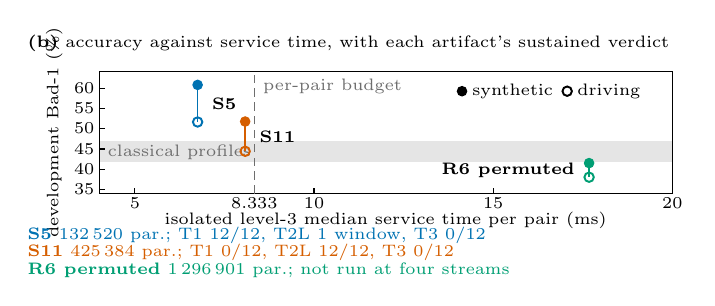
\begin{tikzpicture}[x=1pt,y=1pt,line width=0.4pt]
\definecolor{figblue}{RGB}{0,114,178}
\definecolor{figverm}{RGB}{213,94,0}
\definecolor{figgreen}{RGB}{0,158,115}
\definecolor{figgrey}{RGB}{110,110,110}
\providecommand{\fsix}{\fontsize{6}{7}\selectfont}
\fill[black!10] (26.00,11.27) rectangle (233.15,18.87);
\draw[draw=black] (26.00,0.00) rectangle (233.15,44.00);
\node[anchor=west,inner sep=1.5pt,font=\fsix,text=figgrey] at (27.50,15.07) {classical profiles};
\draw[draw=black] (26.00,1.47) -- (28.00,1.47);
\node[anchor=east,inner sep=1.5pt,font=\fsix] at (26.00,1.47) {35};
\draw[draw=black] (26.00,8.80) -- (28.00,8.80);
\node[anchor=east,inner sep=1.5pt,font=\fsix] at (26.00,8.80) {40};
\draw[draw=black] (26.00,16.13) -- (28.00,16.13);
\node[anchor=east,inner sep=1.5pt,font=\fsix] at (26.00,16.13) {45};
\draw[draw=black] (26.00,23.47) -- (28.00,23.47);
\node[anchor=east,inner sep=1.5pt,font=\fsix] at (26.00,23.47) {50};
\draw[draw=black] (26.00,30.80) -- (28.00,30.80);
\node[anchor=east,inner sep=1.5pt,font=\fsix] at (26.00,30.80) {55};
\draw[draw=black] (26.00,38.13) -- (28.00,38.13);
\node[anchor=east,inner sep=1.5pt,font=\fsix] at (26.00,38.13) {60};
\draw[draw=black] (38.95,0.00) -- (38.95,2.00);
\node[anchor=north,inner sep=1.5pt,font=\fsix] at (38.95,0.00) {5};
\draw[draw=black] (82.10,0.00) -- (82.10,2.00);
\node[anchor=north,inner sep=1.5pt,font=\fsix] at (82.10,0.00) {8.333};
\draw[draw=black] (103.68,0.00) -- (103.68,2.00);
\node[anchor=north,inner sep=1.5pt,font=\fsix] at (103.68,0.00) {10};
\draw[draw=black] (168.41,0.00) -- (168.41,2.00);
\node[anchor=north,inner sep=1.5pt,font=\fsix] at (168.41,0.00) {15};
\draw[draw=black] (233.15,0.00) -- (233.15,2.00);
\node[anchor=north,inner sep=1.5pt,font=\fsix] at (233.15,0.00) {20};
\draw[figgrey,densely dashed] (82.10,0.00) -- (82.10,44.00);
\node[anchor=north west,inner sep=1.5pt,font=\fsix,text=figgrey] at (83.60,43.00) {per-pair budget};
\node[anchor=north,inner sep=0pt,font=\fsix] at (129.57,-6.50) {isolated level-3 median service time per pair (ms)};
\node[rotate=90,anchor=south,inner sep=0pt,font=\fsix] at (13.00,22.00) {development Bad-1 (\%)};
\draw[figblue,line width=0.5pt] (61.61,39.28) -- (61.61,25.87);
\filldraw[fill=figblue,draw=figblue] (61.61,39.28) circle (1.7pt);
\draw[figblue,line width=0.7pt] (61.61,25.87) circle (1.7pt);
\node[anchor=west,inner sep=1.5pt,font=\fsix] at (65.11,32.58) {\textbf{S5}};
\draw[figverm,line width=0.5pt] (78.79,26.04) -- (78.79,15.29);
\filldraw[fill=figverm,draw=figverm] (78.79,26.04) circle (1.7pt);
\draw[figverm,line width=0.7pt] (78.79,15.29) circle (1.7pt);
\node[anchor=west,inner sep=1.5pt,font=\fsix] at (82.29,20.67) {\textbf{S11}};
\draw[figgreen,line width=0.5pt] (203.07,11.02) -- (203.07,5.92);
\filldraw[fill=figgreen,draw=figgreen] (203.07,11.02) circle (1.7pt);
\draw[figgreen,line width=0.7pt] (203.07,5.92) circle (1.7pt);
\node[anchor=east,inner sep=1.5pt,font=\fsix] at (199.57,8.47) {\textbf{R6 permuted}};
\node[anchor=west,inner sep=0pt,font=\fsix,text=figblue] at (0.0,-15.00) {\textbf{S5}\ 132\,520 par.; T1 12/12, T2L 1 window, T3 0/12};
\node[anchor=west,inner sep=0pt,font=\fsix,text=figverm] at (0.0,-21.40) {\textbf{S11}\ 425\,384 par.; T1 0/12, T2L 12/12, T3 0/12};
\node[anchor=west,inner sep=0pt,font=\fsix,text=figgreen] at (0.0,-27.80) {\textbf{R6 permuted}\ 1\,296\,901 par.; not run at four streams};
\filldraw[fill=black,draw=black] (157.15,37.00) circle (1.7pt);
\node[anchor=west,inner sep=2pt,font=\fsix] at (158.65,37.00) {synthetic};
\draw[black,line width=0.7pt] (195.15,37.00) circle (1.7pt);
\node[anchor=west,inner sep=2pt,font=\fsix] at (196.65,37.00) {driving};
\node[anchor=south west,inner sep=0pt,font=\fsix] at (0.0,51.00) {\textbf{(b)}\ accuracy against service time, with each artifact's sustained verdict};
\end{tikzpicture}
